\documentclass[conference]{IEEEtran}
\IEEEoverridecommandlockouts
\usepackage{cite}
\usepackage{xcolor}
\usepackage{mathtools}
\usepackage{footnote}
\usepackage{cancel}
\usepackage{xfrac}
\usepackage{amsmath,amssymb,amsfonts,amsthm}
\usepackage{algorithm}
\usepackage{algorithmicx}
\usepackage{algpseudocode}
\usepackage[hidelinks]{hyperref}
\usepackage{siunitx}
\usepackage{graphicx}
\usepackage{float}
\usepackage{tikz}
\usepackage{textcomp}
\usepackage[utf8]{inputenc}
\usepackage[english]{babel}

\usetikzlibrary{automata, positioning, arrows}
\newtheorem{theorem}{Theorem}

\def\BibTeX{{\rm B\kern-.05em{\sc i\kern-.025em b}\kern-.08em
    T\kern-.1667em\lower.7ex\hbox{E}\kern-.125emX}}

\hypersetup{colorlinks=false}

\begin{document}

\title{Segregation without Computation}

\author{
  \IEEEauthorblockN{Peter Mitrano\IEEEauthorrefmark{1} , Jordan Burkland\IEEEauthorrefmark{1}, Michael Giancola\IEEEauthorrefmark{1}, Carlo Pinciroli\IEEEauthorrefmark{1}}
  \IEEEauthorblockA{\IEEEauthorrefmark{1}Worcester Polytechnic Institute, Worcester, Massachusetts}
}

\maketitle

\begin{abstract}
  In this paper, we demonstrate that robots which directly map one of three sensor readings to wheel speeds, no explicit communication, and have one trivial sensor are capable of $n$-class segregation. We evolve controllers with a genetic algorithm and perform a grid search over all parameters to understand the full parameter space. We analyze two distinct controllers that segregate, one of which is efficient, and prove that aggregation of kin robots is guaranteed when reasonable conditions are met. More broadly, this is an example of how to search for and study emergent behaviors in swarms of simple robots.
\end{abstract}

\begin{IEEEkeywords}
  swarm robotics, robot aggregation, robot segregation
\end{IEEEkeywords}

\section{Introduction and Related Work}

  Many prior methods have demonstrated the ability to aggregate robots and objects in a distributed way\cite{shlyakhov_survey_2017}, and \cite{gauci_self-organized_2014}\cite{gauci_clustering_2014} have shown the ability to perform such tasks with limited computation and sensing capabilities . Segregation is the sorting of robots of different classes into clusters or groups, and is a natural extension of aggregation. Segregation can be seen as a precursor to object sorting, task allocation, or self-assembly. For example, swarms may need to split into arbitrary groups to spread out and search different areas, or segregate by skill or capability in order to form useful heterogeneous teams. Furthermore, we attempt to achieve segregating themselves into an arbitrary number of groups with no messaging between robots, no complex sensors, no leaders or beacons, and no environmental cues.

  In nature, we can find a few examples of aggregation and segregation. Segregation occurs in cells during embryogenesis \cite{batlle_molecular_2012}, and segregation of objects can be found in ants who sort their brood \cite{santos_segregation_2014}. These examples motivate the study of simple controllers for segregation, but our main motivation comes from the broader question of whether a complex behavior like $n$-class segregation can be achieved with a simple robot and controller.

  We make no claims that the controllers studied here are the most practical engineering solutions, but rather that they are an example of how complex behavior can emerge from simple rules. The advantages of simple robots is that they are inexpensive, easier to implement. It is also easy to understand and construct proofs about the behavior of these simple robots and their controllers.

  We also provide analysis of a specific emergent behaviors that allows the segregation to work. This analysis, while specific to the segregation behavior and controllers we found, is an example of how to make provable claims about emergent behavior of simple controllers. This is important because having guarantees on swarm behavior and well understand limitations allows one to make an informed decision about whether to deploy the controller in untested environments. If swarm robotics are to actually be used in disaster relief, as is so often proposed, it's important to know the conditions under which certain behavior is guaranteed. In these scenarios, using the simplistic robot and controllers may actually be advantageous.

  \subsection{Aggregation and Segregation}

    Aggregation is defined as having all robots in the swarm collect at a particular location in a distributed manner. Many swarm aggregation controllers require robots to compute bearing and distance to other robots, to sense gradients in the environment, or to otherwise communicate information. However, implementing these communication systems is difficult in practice, so methods that do not require communication or complex sensing are desirable. In \cite{gauci_self-organized_2014}, the authors propose a new class of controllers that require no computation.

   Gasparri et al. instead develop an aggregation controller which enables robots to respond to guidance commands -- i.e., a human using hand gestures to indicate which direction the swarm should move \cite{gasparri_swarm_2012}. They show that swarms running their controller are able to follow guidance commands and stay aggregated without colliding. A simpler controller is used by Bahgeci and Sahin \cite{bahgeci_evolving_2005}, where robots are equipped with IR distance sensors surrounding the robot, 4 microphones, and an omni-directional speaker. The controller is a linear combination of the IR sensor values and the intensity values of the microphones. The authors show that a genetic algorithm is able to find weights for the controller such that robots aggregate. In \cite{ando_distributed_1999}, the authors present an aggregation controller with very limited sensing and no memory, but allows the robots to perform computations to determine their next position. They prove that their controller is correct in theory, then run the controller in simulation.

    Finally, Gauci et al. consider a binary sensor that maps directly to wheel velocities \cite{gauci_self-organized_2014}. The authors demonstrate extremely robust aggregation despite these limitations, and they also prove formally that aggregation is guaranteed and find theoretical bounds on aggregation time in simple situations. Gauci et al. also perform object aggregation, as opposed to robot aggregation, with the same restrictions on sensing and control \cite{gauci_clustering_2014}.

    Segregation of robots has received little attention in swarm robotics, however many researchers have focused on sorting of objects \cite{vardy_accelerated_2012} \cite{holland_collective_1998} \cite{tao_wang_collective_2004} \cite{holland_stigmergy_1999}. Santos et al. shares our objective, however they assume that each class has the same number of robots and that each robot knows the position of all other robots \cite{santos_segregation_2014}. In contrast, we adhere to the memoryless computeless controller architecture with a simple ternary sensor. \cite{gross_segregation_2009} also explores segregation robots based on local interactions inspired by gravity, however they require a centralized broadcast or a consensus algorithm to agree on the source or direction of gravity.

    %By analysing all the various controllers that we found which perform segregation, we can say that they can all be described by simple rules based on the wheel speeds. These rules are therefore also useful because they tell us something fundemental about the segregation behavior.

  \subsection{Robots That Do Not Compute}

    The memoryless and computeless controllers originally proposed by Gauci et al. has been extended to other tasks and been modified in many ways by other researchers.

    Kernbach et al. propose an aggregation controller roughly based on observations of bees clustering in an optimal temperature location \cite{kernbach_re-embodiment_2009}. In their method, robots are only able to distinguish between collisions between another robot or a wall, can only sense the intensity of a light source when they have collided, and do not communicate information. Although the robots have limited sensing and communication capabilities, the authors show that robots can aggregate to an optimal light intensity location, and that the time to converge to the optimal location improves with increasing number of robots in the environment.

    Robots that do not compute and are memoryless have also been shown to aggregate around a specific object, circle in a ring around an object, and forage for obstacles \cite{johnson_evolving_2016}. In this work, the Johnson and Brown show one can construct simple cost functions to guide the evolution of controllers to do new, yet interesting tasks. However, they also report that in attempting to evolve a controller to rendezvous the robots around an object, they accidentally and consistently evolved a controller where the robots circled around the target object. They achieved rendezvous by initializing the controller at generation zero to the controller found in \cite{gauci_self-organized_2014} for simple aggregation.

\section{Methodology}

  \subsection{Problem Formulation}

    We consider a collection of differential drive robots all executing the same controller in a homogeneous, two dimensional, obstacle free environment. The robots are equipped with a single forward facing line of sight sensor which can distinguish between the presence of a kin robot, a non-kin robot, and the absence of a robot. This sensor is assumed to have infinite length (we consider non-infinite length in Section \ref{section:beam_length}). We assign $I=0$ to the state when no robot is seen, $I=1$ to the detection of a kin robot, and $I=2$ to the detection of a non-kin robot. We allow for any number of classes, but the robots need not distinguish between different non-kin classes. They need only to detect if a robot is of the same class or not. The objective is to segregate robots into clusters, ideally such that all the robots of the same class are packed into one cluster with no non-kin robots.

    \begin{algorithm}[t!]
      \begin{algorithmic}
      \If {$I=0$} \State set wheel speeds to $v_{l_0}$, $v_{r_0}$
      \ElsIf {$I=1$} \State set wheel speeds to $v_{l_1}$, $v_{r_1}$
      \Else \State set wheel speeds to $v_{l_2}$, $v_{r_2}$
      \EndIf
      \end{algorithmic}
      \caption{Controller Design}
      \label{alg:controller}
    \end{algorithm}

    The controllers we use in our experiments are of the same form as in \cite{gauci_self-organized_2014}. The controller maps each of the three sensor values to a set of wheel speeds. Pseudo-code for the controller is shown in Algorithm \ref{alg:controller}. This controller has six parameters:

    $$[\,v_{l_0}, v_{r_0}, v_{l_1}, v_{r_1}, v_{l_2}, v_{r_2}\,]$$

    Keeping with the form used in \cite{gauci_self-organized_2014}, we let these parameters range from -1 to 1. In simulation, we then scale this parameter to range from \SI{-20}{\centi\meter\per\second} to \SI{20}{\centi\meter\per\second}.

  \subsection{Simulation Environment}

    We use the ARGoS simulation environment to search for controller parameters and evaluate them, which has the advantage of allowing us to run trials much faster than on real robots \cite{pinciroli_argos:_2012}. In our simulations, we use a range-and-bearing sensor to implement the theoretical line of sight sensor. In our analysis, we describe the sensor as infinitely thin, but in practice it must have some small finite angle. We explore the performance effect of various beam angles in Section \ref{section:beam_angle}. We note here the detail that we consider robots to be connected in a cluster if the gap between them is \SI{5}{\centi\meter} or less. We now describe two approaches for finding these parameters, genetic algorithms and grid search.

  \subsection{Evolving Segregation}

    \cite{bahgeci_evolving_2005}\cite{johnson_evolving_2016}\cite{dorigo_evolving_2004} show that evolutionary strategies are effective for finding emergent behavior. In order to quickly search for parameters to achieve segregation, we use a simple genetic algorithm to evolve controller parameters. The genetic algorithm we used is unmodified from the example MPGA code\footnote{http://www.argos-sim.info/examples.php} provided with the ARGoS simulator. The mutation strategy is to mutate each of these 6 parameters with some probability $p$ ($0.05$ in our experiments). If a parameter is selected to be mutated, a uniformly random number from -1 to 1 is picked for the new value. Selection is performed by picking the two lowest cost individuals, and the next population is formed by crossing the parameters of these two individuals. The original two parents are always kept in the population so that the current lowest cost individual is never removed until a lower cost genome is discovered.

  \subsection{Cost Functions}

    As with any optimization algorithm, it is important to have a cost function that accurately assigns cost to behaviors. We explore two different cost functions, and we find that one of them did not behave as we expected (see Section \ref{section:evaluting_cost_functions}). The first cost metric, shown in Equation \eqref{eq:cluster_cost}, is based on the cluster metric $c_{\text{gauci}}^{(t)}$ used by \cite{gauci_self-organized_2014}, which is the proportion of the number of robots in the largest cluster to the total number of robots at some time step $t$.

    \begin{equation} \label{eq:cluster_cost}
      c_{\text{total}} =  \frac{1}{n}\sum^n\sum_{t=0}^{T-1} -t c_{\text{gauci}}^{(t)}
    \end{equation}

    Let $n$ be the number of classes of robots, and $T$ be the total number of time steps in the trial being evaluated. We apply this cost function for each class of robots and sum the cluster-metric cost for each class to get the total cost. The negative sign is present because the cluster metric is 0 when no robots are connected and 1 when all robots in a class are connected, so the negative sign assigns more connections a lower cost. We used this cost function in grid search and all following experiments.

    The cluster metric in \eqref{eq:cluster_cost} is problematic because it considers a straight line of robots to be one cluster. For some tasks like task allocation, we might care about how tightly the swarm is packed in its clusters. Therefore, we also experiented with a second cost metric. This new metric uses the centroids of the robots in each class. We borrow the dispersion metric $u^{(t)}$ from \cite{gauci_self-organized_2014}, which essentially computes the sum of distances from each robot to the centroid, but in our case we apply this to each class of robots. Consider $u_i^{(t)}$ to be the dispersion of a particular class $i$ at time $t$. Given all the centroids $\bar{p}_i^{(t)}$ for each class $i$, we call the centroid of all of these centroids $\bar{P}^{(t)}$. First, let $c_{\text{intra}}$ be the total cost of dispersion within all the classes of robots, which should be low because robots within the same class should be close to one another. $c_{\text{intra}}$ is then the cost of the dispersion of the centroids, which should be high because we want the clusters kin robots to be far apart. We call this the centroid-of-centroids cost function $c_{\text{total}}$, and it is defined formally in Equation \eqref{eq:centroid_cost}.

    \begin{equation} \label{eq:centroid_cost}
      \begin{split}
        u_i^{(t)} &= -\frac{1} {4r^2}\sum_{j=1}^{m_{i}}{\lVert p_{i,j}^{(t)} - \bar{p}_{i,j}^{(t)} \rVert}^2 \\
        c_{\text{intra}} &= \sum_{i=1}^n u_i^{(t)} \\
        c_{\text{inter}} &= -\frac{1} {4r^2}\sum_{i=1}^n{\lVert \bar{p}_i^{(t)} - \bar{P}_i^{(t)} \rVert}^2 \\
        c_{\text{total}} &=  \sum_{t=0}^{T-1} t (c_{\text{intra}} + c_{\text{inter}}) \\
      \end{split}
    \end{equation}

    Let $m$ be the number of robots in group $i$, $T$ be the total number of time steps, $t$ be a specific time step, $n$ be the total number of classes, $r$ be the radius of the robot.

  \subsection{Grid Search}

    In order to exhaustively search the space of possible controllers, we conducted a grid search of the 6-dimensional parameter space. Due to limited computational resources, we were only able to search with a resolution of 7 values per parameter, which means in total we evaluated $7^6=117649$ parameters. For each parameter, we ran 1 trial in 36 different initial configurations, with 180 seconds for each simulation. These configurations consisted of uniformly random placement, clusters, and lines of robots distributed throughout the environment. We chose to include some structure configurations (clusters and lines) because we discovered that they varied significantly in performance from uniform random configurations, and by explicitly evaluating on structure configurations we can speak more confidently about the ability of the controller to succeed in any configuration. Otherwise, we would need to have far more trials with uniformly random robot placement to make the same claims. We were able to parallelize across the 36 configurations and run at 75x real time, so it took approximately 4 days to evaluate all the controllers.

    Because the search space is six-dimensional, we chose to visualize it by plotting every pair of parameters against each other. For example, we consider how the cost changes as $v_{l_0}$ and $v_{r_0}$ change. We note that these graphs, shown in Appendix \ref{section:grid_search_images}, show very similar patterns to the same plots presented by \cite{gauci_self-organized_2014}. As an example of reading these plots, we can tell from the plot of parameters 2 and 3 ($I=1$) that there were no good controllers where the left and right wheel speeds were equal and negative (dark squares in the upper left), and that the best controllers had slightly unequal values close to 1 (lightest squares in the bottom left). These plots also visualize how there are some sharp discontinuities where performance changes dramatically.

\section{The Emergent Behavior}

    After running 10 generations with 10 genomes per generation, the lowest cost controller found was [0.5, -0.5, -0.2, 0.6, 0.6, 0.2]. Similarly, after running the grid search, the best controller was [1, -$\sfrac{2}{3}$, $\sfrac{1}{3}$, 1, 1, 0]. For both of these controllers, the resulting behavior is to turn away from kin but turn the opposite way when they see nothing or non-kin. This behavior causes the kin robots to zig-zag in a line towards their kin, and when multiple robots execute this behavior the kin robots form rings. An example of this can be seen in Figure \ref{fig:rings}. Rarely, the robots form shrimp-like shapes which can also be seen in Figure \ref{fig:rings}.

    \begin{figure}
      \centering
      \includegraphics[width=0.7\linewidth]{./images/rings_example.png}
      \caption{the emergent behavior is rings of kin. These rings expand and drift over time.}
      \label{fig:rings}
    \end{figure}

    The dynamics of the robots is far more complex than merely forming rings. A complete description of the observed behavior is beyond the scope of this paper, but we encourage the curious reader to view the supplementary videos at \href{https://www.youtube.com/playlist?list=PL9HqYJ1IkIKVX9EsT5BY9LnBsBPTjc5bB}{https://goo.gl/z8UAuB}. For example, we notice that the rings, once formed, expand over time. If a ring is disturbed by non-kin robots that trying to pass through, the ring is disrupted and eventually reforms.

\section{Controller Analysis}

  We found from grid search that the parameters [$1$, $-0.6667$, $0.3333$, $1.0$, $1.0$, $0.0$] best achieve segregation as defined by our cluster metric cost function. The actual wheel speeds, which are scaled by $0.2$ to convert to \SI{}{\meter\per\second} are therefore [$0.2$, $-0.1333$, $0.06667$, $0.2$, $0.2$, $0.0$]. Now that we have found parameters that achieve what we consider segregation, we define the conditions under segregation is guaranteed. We first prove that aggregation between two isolated kin robots is guaranteed under weak assumptions. Then we show that kin will aggregate with a static ring of kin. Furthermore, we explain why groups of three or more robots usually form rings. Finally, we show that non-kin will aggregate faster to kin than non-kin. All together, this explains much of the emergent behavior. More generally it demonstrates that we can prove useful things about complex emergent swarm behavior of these simple robots and controllers. In all of these proofs we will consider the controller found via grid search since it is the best controller. We also assume the controllers are in sync, that each motion is execute for the same $\Delta t$ at the same point in time, and that the robot has a fixed positive inter wheel distance $W$ and radius $r$.

    \begin{figure}[t!]
      \centering
      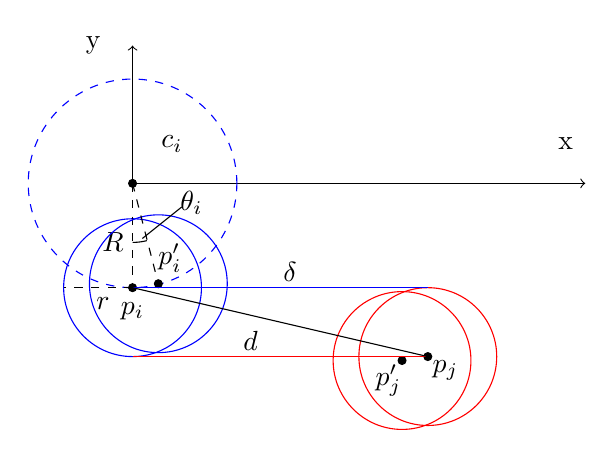
\begin{tikzpicture}[scale=25.0]
        \draw[->] (0,0) -- (0.23,0);
        \node at (0.22,.02) {x};
        \draw[->] (0,0) -- (0,0.07);
        \node at (-.02,0.07) {y};

         % c_i
        \filldraw (0,0) circle (.002);
        \node at (.02,.02) {$c_i$};
        \draw[blue, dashed] (0,0) circle (0.053);

         % p_i
        \filldraw (0,-0.053) circle (.002);
        \node at (0,-0.065) {$p_i$};
        \draw[blue] (0,-.053) circle (0.035);
        \node at (-0.01,-.03) {$R$};
        \draw[dashed] (0,0) -- (0,-0.053);
        \draw[dashed] (0,-0.053) -- (-0.035,-0.053);
        \node at (-0.015,-0.061) {$r$};

         % p'_i
        \filldraw (0.0131,-0.051) circle (.002);
        \node at (0.019,-0.038) {$p'_i$};
        \draw[blue] (0.0131,-0.051) circle (0.035);
        \draw[dashed] (0,0) -- (0.0131,-0.051);

         % p_j
        \filldraw (0.15, -0.088) circle (.002);
        \node at (0.159, -0.095) {$p_j$};
        \draw[red] (0.15, -0.088) circle (0.035);

         % p'_j
        \filldraw (0.1369, -0.09) circle (.002);
        \node at (0.13, -0.1) {$p'_j$};
        \draw[red] (0.1369, -0.09) circle (0.035);

        % delta
        \draw[blue] (0,-.053) -- (.15,-.053);
        \draw[red] (0,-.088) -- (.15,-.088);
        \node at (0.08, -0.045) {$\delta$};

        % theta
        \draw (0,-.03) arc [radius=.03, start angle=-90, end angle=-76];
        % TODO add theta annotation back
        \node at (.03,-.01) {$\theta_i$};
        \draw (.025,-.012) -- (.005, -.028);

        % d
        \draw (0,-0.053) -- (0.15, -0.088);
        \node at (0.06,-0.08) {$d$};
      \end{tikzpicture}
      \caption{The configuration of a robot aggregating to another kin where both robots see each other. $R$ is the radius of the robots path around the ICC.}
      \label{fig:kin_aggregation}
    \end{figure}

  \subsection{Aggregation of Two Kin}

    \begin{figure}[t!]
      \centering
			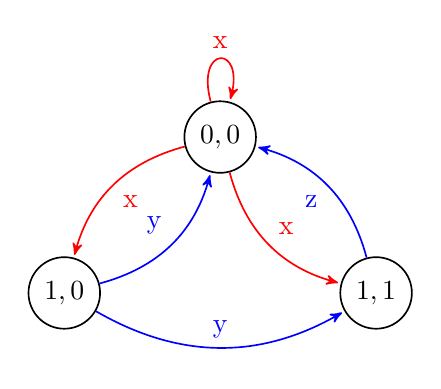
\begin{tikzpicture}[->,>=stealth',shorten >=1pt,auto,node distance=2.8cm, semithick]
				\node[state] (A)                    {$0,0$};
				\node[state] (B) [below left of=A]  {$1,0$};
				\node[state] (C) [below right of=A] {$1,1$};
        \node at (0, -2.5) (hidden) {};

				\path (A) edge [red, loop above] node {x} (A)
                  edge [red, bend right] node {x} (B)
                  edge [red, bend right] node {x} (C)
              (B) edge [blue, bend right] node {y} (C)
                  edge [blue, bend right] node {y} (A)
              (C) edge [blue, bend right] node {z} (A);
			\end{tikzpicture}
      \label{fig:fsm}
      \caption{State machine representation for two kin aggregation. (1,0) means robot $i$ has sensor state $I=0$, and robot $j$ has $I=1$. Blue arrows indicate transitions where the robots aggregate, and red indicates they may not aggregate. Letters indicate identical transitions. One can see visually in Figure \ref{fig:kin_aggregation} why it's impossible to transition from $1,1$ to $1,0$.}
		\end{figure}

    The set of all possible initial configurations of two robots $i$ and $j$ can be split into three possible states. Either neither robot sees the other, one robot sees the other, or both robots see each other. In order to show that aggregation is guaranteed in all scenarios, we consider how these states evolve as a finite state machine (Figure \ref{fig:fsm}). For each sensor state $I=0,1,2$ there is a corresponding radius of rotation around the ICC which we call $R_0$, $R_1$, $R_2$ respectively. There are three unique transitions between states in this state machine, which are called $x$, $y$ and $z$.

    We show that the distance by which the robots aggregate during the blue transitions $y$ or $z$ is always greater than the distance they could possibly separate in any sequence of $x$ transitions. The upper bound on how much the robots disperse in transition $x$ we call $s$, and it is equal to twice the radius of the curvature of the robots path $R_0$. Equation \eqref{eq:s_bound} formally defines $s$.

    \begin{equation} \label{eq:s_bound}
      \begin{split}
        s &= 2R_0 = 2\frac{W}{2}\bigg(\frac{v_{l_1} + v_{r_1}}{v_{l_1} - v_{r_1}}\bigg) = \frac{W}{4}\bigg(\frac{0.2 + -0.133}{0.2 - (-1.333)}\bigg) \\
        &= 0.8W
      \end{split}
    \end{equation}

    We need to show that, in transitions $y$ and $z$, the kin robots always aggregate more than $s$. We first demonstrate that the magnitude of aggregation, which can be described as $d'-d$ in Figure \ref{fig:kin_aggregation}, always increases as $\delta$ increases. In other words, the closer the robots are, the less by which they aggregate. The conditions under which this is true are derived in Equation \ref{thm:d-d}. Given this fact, if we can then also prove that the robots aggregate by more than $s$ at the smallest $\delta$, then they must also aggregate for all $\delta$. This second condition is derived in Equations \ref{thm:one_see_cond} and \ref{thm:both_see_cond}, and the final conditions are shown below. We know the lower bound of $\delta$ is $\sqrt{2}r$ because this is the point at which the two robots are touching.

    \begin{equation} \label{eq:two_kin_cond_1}
        \frac{1}{-W-r+W\cos(\theta_i)} \leq \sqrt{2}
    \end{equation}

    % TODO: maybe mention this second constrain is always true if the third one is
    \begin{equation} \label{eq:two_kin_cond_2}
      \begin{split}
        &\sqrt{(\sqrt{2}r_j - W\sin(\theta_i))^2 + (-W-r_j+W\cos(\theta_i))^2} \\
        & - \sqrt{3}r_j < \frac{\Delta t}{15W} + 1.6W\sin\bigg(\frac{\Delta t}{6W}\bigg)
      \end{split}
    \end{equation}

    \begin{equation} \label{eq:two_kin_cond_3}
      \begin{split}
        &\sqrt{(\sqrt{2}r_j - 2W\sin(\theta_i))^2 + (-r_j-2W+2W\cos(\theta_i))^2} \\
        & - \sqrt{3}r_j < \frac{\Delta t}{15W}
      \end{split}
    \end{equation}

    Ultimately, if Equations \eqref{eq:two_kin_cond_1}, \eqref{eq:two_kin_cond_2}, and \eqref{eq:two_kin_cond_3} are satisfied, we can say that from any initial configuration, two kin robots will eventually aggregate in a sort of two-steps-forward one-step-back fashion. This behavior is clearly demonstrated in our simulation and real robot experiments.

  \subsection{Aggregation with Ring of Kin}

    \begin{theorem} \label{thm:aggregation_with_ring_of_kin}
      An isolated kin robot will aggregate to a ring of kin.
    \end{theorem}
    \begin{proof}

      In this scenario, imagine a isolated kin robot which has sensed a ring of kin. If we consider the center of the ring static, we can extend Theorem \ref{thm:one_robot_sees_the_other} to determine the conditions under which it is guaranteed that the isolated robot will aggregate to the ring of kin. Imagine the ring of kin as robot $j$ but with a different (larger) radius than the isolated robot $i$. In this case, the coordinates of $p_j$ are a function of the new $r_j$ which no longer necessarily equals $r$. Following the same process, the condition in Equation \eqref{eq:ring_agg} described when aggregation is guaranteed.

      \begin{equation} \label{eq:ring_agg}
        \begin{split}
          beep boop
        \end{split}
      \end{equation}

      \end{proof}

     Shown in Figure \ref{fig:kin_aggregation}. The controller dictates that since a kin robot is seen, $I=1$, so $v_{l_1} = 0.3333$ and $v_{r_1} = 1$. This will cause the robot to turn counter-clockwise with some radius $R_1$. Our goal is to show that the robots will always be closer after executing the controller. Like in our proof of two kin aggregation, we want to show that the robot and the other kin are closer after executing the controller (see Equation \eqref{eq:agg}).

    With this coordinate system defined, we can define the coordinates of $p_i$, $p_j$, and $p'_i$ (Equation \eqref{eq:vars}). Next, we can write the variables $\theta_i$ and $R_1$ in terms of $\Delta t$, the inter wheel diameter $W$, and the wheels speeds of the controller $v_{l_1}$ and $v_{r_1}$, which are shown in Equation \eqref{eq:theta_and_r}.

    We then substitute these variables into Equation \eqref{eq:agg} and simplify, and the result is shown in Equation \eqref{eq:agg_result}. For the full derivation, see Appendix \ref{apx:1}. In other words, for aggregation to a static kin robot to be guaranteed, the robot sizes and controller period must meet this condition. Intuitively, the robot or ring radius $r_j$ should not be large compared to the other robot radius $r$, the time step should be small, and $W$ should not be too small. We emphasize that $r_j$ could be the radius of a single kin robot or the radius of a large static ring of kin robots.

    \begin{equation} \label{eq:agg_result}
      \sqrt{r^2_i + 2rr_j} > (W+r_j)\tan{\frac{\Delta t}{15W}}
    \end{equation}

    Equation \eqref{eq:agg_result} is useful because it tells us whether aggregation is guaranteed knowing only the sizes of the robots and the largest ring we expect to form. This condition may not hold true for all scenarios (such as those with thousands of small robots or large $\Delta t$), but we show it holds true for many popular robots in Table \ref{table:robots}. This table shows that largest ring size $r_j$ for which aggregation is guaranteed, assuming a controller period of \SI{0.1}{\second}. The maximum size of $r_j$ can be computed analytically as we show in Appendix \ref{apx:1}. From this table, we can see that the controller speeds are most effective on the foot-bot, which is expected because our grid search used the foot-bot.

    \begin{savenotes}
    \begin{table}
      \centering
      \caption{Aggregation is guaranteed for many differential drive swarm robots.}
      \begin{tabular}{|c|c|c|c|} \hline
        Robot & $r$ (m) & $W$ (m) & maximum $r_j$ (m) \\ \hline
        foot-bot\footnote{\href{https://github.com/ilpincy/argos3/blob/master/src/plugins/robots/foot-bot/simulator/footbot_entity.cpp}{ARGoS file footbot\_entity.cpp}} &
            0.085 & 0.14 & 74.619 \\ \hline
        Khephera IV\footnote{Khephera IV User Manual, page 66.} &
            0.07 & 0.1054 & 34.725 \\ \hline
        E-Puck 2\footnote{\href{http://projects.gctronic.com/epuck2/e-puck2-flyer.pdf}{http://projects.gctronic.com/epuck2/e-puck2-flyer.pdf}} &
            0.035 & 0.053 & 4.288 \\ \hline
        Kilobot\footnote{\href{https://www.k-team.com/mobile-robotics-products/kilobot/specifications}{https://www.k-team.com/mobile-robotics-products/kilobot/specifications}} &
            0.0165 & 0.030\footnote{only approximate} & 0.594 \\ \hline
      \end{tabular}
      \label{table:robots}
    \end{table}
    \end{savenotes}

    Ultimately, we can use these geometric proof to make a useful assertions about the behavior of an individual in our swarm and of the swarm as a whole. While we have not shown that segregation is guaranteed in all cases, this may serve as a building block for more general claims.

\section{Experimental Results}

  \subsection{Evaluating the centroid-of-centroids cost function} \label{section:evaluting_cost_functions}

    When we implemented the centroid-of-centroids style cost function, we quickly found examples of configurations which were ranked undesirably. One example is shown below in Figure \ref{fig:cost_function_fuckup}. The behavior that looks like aggregation was given lower cost of $-8\cdot 10^{9}$, versus the behavior that looks like segregation was given a cost of $-5\cdot 10^{9}$.

    \begin{figure}[H]
      \centering
      \includegraphics[width=0.49\linewidth]{./images/individual_0_gen_0.png}
      \includegraphics[width=0.49\linewidth]{./images/individual_0_gen_1_better.png}
      \caption{The left picture was given lower cost than the right, which is not desirable.}
      \label{fig:cost_function_fuckup}
    \end{figure}

  \subsection{Scalability Study} \label{section:scalability}

    In this experiment we investigate how segregation behavior scales with the number of classes and number of robots in the environment. We varied the number of classes from 1 to 25 and ran 100 trials of robots uniformly randomly distributed.

    \paragraph{Fixed number of robots per class}

    Because our cost function is independent of the number of classes, we first considered having 10 robots for each class. However, this also means that in the trial with 25 classes there are 25 times the total number of robots than in the 1-class trial. This means that occlusion of robots is more likely and so the cost increases with more classes. The results of this are plotted in Figure  \ref{fig:num_classes_10}.

    \paragraph{Fixed total number of robots}

    Another scenario is to consider a fixed number of robots and split them into more and more classes. We choose 100 robots because we are still able to get 4 robots per class at 25 classes. As you can see in Figure \ref{fig:num_classes_100}, the cost no longer increases as the number of classes increases. However, the cost for just a few classes is much higher. This is expected, because when there are many robots of a single class, our controller forms very large sparse rings where robots are too far apart to be considered clustered.

    Ultimately, we can say that our controller scales well to many classes with few robots, but not well to many robots of the same class.

    \begin{figure}[H]
      \centering
      \includegraphics[width=1\linewidth]{./images/num_classes_vs_cost_100_robots.png}
      \caption{The average cost with 100 robots divided into N classes. More classes are lower cost partially because kin robots stay close enough to be considered clusters.}
      \label{fig:num_classes_100}
    \end{figure}

    \begin{figure}[H]
      \centering
      \includegraphics[width=1\linewidth]{./images/num_classes_vs_cost_10_per_class.png}
      \caption{The average cost with N classes, 10 robots per class. More classes are higher cost because other robots obstruct your view making it difficult to find kin.}
      \label{fig:num_classes_10}
    \end{figure}

  \subsection{The Effect of Implementation Details of the sensor} \label{section:sensor_impl}

    We found in our experiments that the implementation details of the line-of-sight sensor have a significant effect on the behavior of the controller.

    Initially, our method for determining sensor state from our simulated range-and-bearing sensors was to consider all the robots within some small angle in front of the robot and pick the closest one. This is very similar to what would be provided by a real-world camera that uses colored skirts on each robot and picks the largest blob as the robot to be detected. This sensor implementation works well and was used in all our genetic algorithm and grid search experiments. However, we found later that if the robots instead always prefer to react to kin over non-kin, you can form larger rings more quickly and robustly. For example, if there are two robots within the field of view of your sensor and the non-kin robot is closer, you will ignore it and execute the $I=1$ state which will drive you towards the farther away kin robot. Exploring exactly which of these implementation details have what effect on cost is left for future work.

  \subsection{The Effect of the Beam Angle} \label{section:beam_angle}

    On a real robot, there must be some finite beam angle to the theoretically line-of-sight sensor. We ran 100 trials in simulation with uniformly random initial distributions of 40 robots with various half beam angles. Figure \ref{fig:beam_angle} shows the results, as well as a diagram showing how we define half beam angle. The best half beam angle we tested was \ang{15}, and angles smaller or larger became progressively worse. We found that at lower beam angles, it was possible for a robot to become stuck in groups of two or three where the robots spent all their time looking at each other and not peeking around them to find kin. At larger angles, we believe the behavior fails because larger beam angles cause the rings to enlarge faster, which in turn causes the rings to be so large that they are not considered a cluster anymore and so the cost rises.

    \begin{figure}[H]
      \centering
      \includegraphics[width=1\linewidth]{./images/beam_angle.png}
      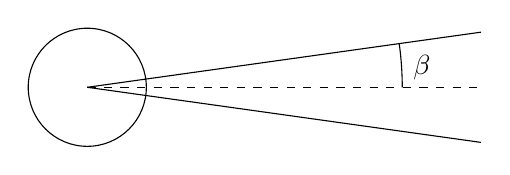
\begin{tikzpicture}
        \draw (0,0) circle (0.75);
        \draw (0,0) -- (5,0.7);
        \draw[dashed] (0,0) -- (5,0);
        \draw (0,0) -- (5,-0.7);
        \draw (4,0) arc [radius=4, start angle=0, end angle=8];
        \node at (4.25,0.25) {$\beta$};
      \end{tikzpicture}
      \caption{A \ang{15} degree half beam angle is best for segregation. Lower cost is better.}
      \label{fig:beam_angle}
    \end{figure}

  \subsection{The Effect of Beam Length} \label{section:beam_length}

    We also consider what happens if our theoretically infinite sensor now has finite range. We use \ang{15} half beam angle and the same experimental setup as with the beam angle experiments. Analogously to \cite{gauci_self-organized_2014}, we consider the maximum range of the sensor as the diagonal length of the square in which the robot are initially distributed. In all our experiments, this box was \SI{5}{\meter\square}, so we consider a range of \SI{7.07}{\meter} to be effectively unlimited. We report the costs for beam lengths as a fraction of this maximum range. As shown in Figure \ref{fig:beam_length}, a beam length of 35\% of the theoretical maximum performs just as well. Below this, the performance degrades. However, even a beam length of 7\% of unlimited is more effective than zero length at segregation. In our experiment watching many simulations, beam length should also be scaled with the total number of robots as well as the initial distance between robots. When the beam length is short, there are many cases where two rings of kin robots form at different points in the environment, and in order for these two rings to join the robots must have sufficiently long beam length in order to detect each other.

    \begin{figure}
      \centering
      \includegraphics[width=1\linewidth]{./images/beam_length.png}
      \caption{Segregation is robust to very finite sensor beam lengths. The blue bar indicates the worst (highest) attainable cost in which all robots are isolated from any kin.}
      \label{fig:beam_length}
    \end{figure}

\section{Conclusion}

  In this paper, we demonstrate that memoryless, computeless robots are capable of $n$-class segregation. We use a simple controller design consisting of a 6-tuple. This controller is invariant to the number of classes, so any given controller can work for any number of classes. To quickly find a quality controller, we evolved one using a basic genetic algorithm, but we also performed a grid search to make claims about the full parameter space. We investigated the effect of sensor implementation details and the number of robots and classes on performance. We find that robust segregation is possible, although not guaranteed. Instead, we prove that aggregation of kin robots is guaranteed when reasonable conditions on controller frequency and inner wheel distance are met.

\bibliography{RBE595.bib}
\bibliographystyle{unsrt}

\onecolumn
\appendix
\section{Appendix}

    \begin{align}
      \begin{split} \label{eq:theta_and_r}
        \theta_i &= \Delta t\omega = \Delta t \frac{v_{r_1} - v_{l_1}}{W} = \Delta t \frac{0.2 - 0.06667}{W} = \frac{2\Delta t}{15W} \\
        R_1 &= \frac{W}{2}\bigg(\frac{v_{r_1} + v_{l_1}}{v_{r_1} - v_{l_1}}\bigg) = \frac{W}{2}\bigg(\frac{0.2 + 0.06667}{0.2 - 0.06667}\bigg) = W
      \end{split}
    \end{align}

    From Figure \ref{fig:kin_aggregation} we can define the coordinates of $p_i$, $p_j$, $p'_i$, and $p'_j$.

    \begin{equation} \label{eq:two_kin_vars_1}
      \begin{split}
        p_i = \begin{bmatrix}0 \\ -R_1\end{bmatrix} \\
        p_j = \begin{bmatrix}\delta \\ -(R_1+r_j)\end{bmatrix} \\
        p'_i = \begin{bmatrix}R_1\sin(\theta_i) \\ -R_1\cos(\theta_i)\end{bmatrix} \\
        p'_j = \begin{bmatrix}\delta - R_1\sin(\theta_i) \\ -(R_1+r) - (R_1-R_1\cos(\theta_i))\end{bmatrix} \\
      \end{split}
    \end{equation}

  \begin{theorem} \label{thm:d-d}
    Robots aggregate by less the closer they are
  \end{theorem}
  \begin{proof}

    We show that $d'-d$ always decreases as $\delta$ increases. This is true if the derivative $\frac{\partial}{\partial\delta}(d'-d) \leq 0$, $\forall \delta>\sqrt{2}r$.

    {%
      \setlength{\belowdisplayskip}{3pt}%
      \setlength{\abovedisplayskip}{3pt}%
      \begin{align*}
        \frac{\partial}{\partial\delta}(d'-d) &< 0 \\
        \frac{\partial}{\partial\delta}\big(\lVert p_j - p'_i \rVert - \lVert p_j - p_i \rVert\big) &\leq 0 \\
        \frac{\partial}{\partial\delta}\bigg(\sqrt{(p_{j_x} - p'_{i_x})^2 + (p_{j_y} - p'_{i_y})^2} - \sqrt{(p_{j_x} - p_{i_x})^2 + (p_{j_y} - p_{i_y})^2}\bigg) &\leq 0 \\
        \frac{\partial}{\partial\delta}\bigg(\sqrt{(\delta - b)^2 + a} - \sqrt{(\delta- 0)^2 + (p_{j_y} - p_{i_y})^2}\bigg) &\leq 0 \\
        \frac{\partial}{\partial\delta}\bigg(\sqrt{(\delta - b)^2 + a} - \sqrt{\delta^2 + (p_{j_y} - p_{i_y})^2}\bigg) &\leq 0 \\
        \frac{\partial}{\partial\delta}\bigg(\sqrt{(\delta-b)^2 + a} - \sqrt{\delta^2 + (-(R_1+r) - R_1)^2}\bigg) &\leq 0 \\
        \frac{\partial}{\partial\delta}\bigg(\sqrt{(\delta-b)^2 + a} - \sqrt{\delta^2 + r^2}\bigg) &\leq 0 \\
        \frac{1}{2}\Big[(\delta-b)^2 + a)^{-\frac{1}{2}}(2\delta-2b) - (\delta^2 + r^2)^{-\frac{1}{2}}(2\delta)\Big] &\leq 0 \\
        ((\delta-b)^2 + a)^{-\frac{1}{2}}(\delta-b) - (\delta^2 + r^2)^{-\frac{1}{2}}(\delta) &\leq 0 \\
        ((\delta-b)^2 + a)^{-\frac{1}{2}}(\delta-b) &\leq (\delta^2 + r^2)^{-\frac{1}{2}}(\delta) \\
        (\delta^2 + r^2)^{\frac{1}{2}}(\delta-b) &\leq (\delta)((\delta-b)^2 + a)^{\frac{1}{2}} && \text{all terms are positive, see Theorem \ref{thm:d-b}} \\
        (\delta^2 + r^2)^{\frac{1}{2}}(\delta-b) &\leq (\delta)((\delta-b)^2 + a)^{\frac{1}{2}} \\
        (\delta^2 + r^2)(\delta-b)^2 &\leq (\delta)^2((\delta-b)^2 + a) \\
        (\delta^2 + r^2)(\delta-b)^2 &\leq (\delta-b)^2(\delta^2 + a\delta^2) \\
        (\delta^2 + r^2) &\leq (\delta^2 + a\delta^2) \\
        r^2 &\leq a\delta^2 \\
        \frac{r}{\sqrt{a}} &\leq \delta \\
        \frac{r}{\sqrt{(-W-r+W\cos(\theta_i))^2}} &\leq \delta \\
        \frac{r}{-W-r+W\cos(\theta_i)} &\leq \delta \\
        \frac{r}{-W-r+W\cos(\theta_i)} &\leq \sqrt{2}r && \text{lower bound on }\delta \\
        \frac{1}{-W-r+W\cos(\theta_i)} &\leq \sqrt{2} \\
      \end{align*}

      We have now shown that if $\frac{1}{-W-r+W\cos(\theta_i)} \leq \sqrt{2}$, then this implies that the change in distance $d'-d$ strictly decreases as $\delta$ increases. In other words, the amount that the two robots get closer is smallest when they are as close as possible. Because of this property, we can guarantee aggregation by showing that $d'-d<s$ when $d$ is at its minimum of $\sqrt{2}r$. In other words, if these two simple analytic conditions are satisfied, than aggregation between two kin robots is guaranteed. For convenience, we show the expanded forms of $d'-d$ for the two possible cases. To apply this, substitute the parameters of your robot into the two equations below and see if the conditions hold true.

    }

  \end{proof}

  \begin{theorem} \label{thm:one_see_cond}
    $d'-d<s$ in state $1,0$ when one robot sees the other.
  \end{theorem}
  \begin{proof}

    In this state, robot $i$ will arc left with speeds $0.06667, 0.2$ and robot $j$ will rotate right with speeds $0.2, -0.1333$. Robot $i$ advances towards $j$ along a slight arc, whereas $j$ rotates mostly in place. Because $j$ is not stationary, there is an additional amount which it could move away from $i$, so in addition to showing that $d'-d<s$ we must add another approximate value to $s$ which we'll call $s'$. This maximum distance $j$ can move in one time step is the length of the chord defined by the radius $R_0$ (radius of turn for sensor $I=0$) and angle $\theta_j$. Equation \eqref{eq:s'} shows the full definition of this bound.

    \begin{equation} \label{eq:s'}
      \begin{split}
        \theta_j &= \Delta t\omega = \Delta t \frac{v_{l_1} - v_{r_1}}{W} = \Delta t \frac{0.2 - (-0.1333)}{W} = \frac{\Delta t}{3W} \\
        s' &= 2R_0\sin\bigg(\frac{\theta_j}{2}\bigg) = 2(0.8W)\sin\bigg(\frac{\Delta t}{6W}\bigg) = 1.6W\sin\bigg(\frac{\Delta t}{6W}\bigg)
      \end{split}
    \end{equation}

    \begin{align*}
      d' - d &< s + s' \\ %TODO (peter) account for the other s' which is from robot J rotating
      \lVert p_j - p'_i \rVert - \lVert p_j - p_i \rVert &< s + s' \\
      \sqrt{(p_{j_x} - p'_{i_x})^2 + (p_{j_y} - p'_{i_y})^2} - \sqrt{(p_{j_x} - p_{i_x})^2 + (p_{j_y} - p_{i_y})^2} &< s + s' \\
      \sqrt{(\sqrt{2}r_j - R_1\sin(\theta_i))^2 + (-(R_1+r_j) - (-R_1\cos(\theta_i)))^2} - \sqrt{(\sqrt{2}r_j - 0)^2 + (-(R_1+r_j) - (-R_1))^2} &< s + s' \\
      \sqrt{(\sqrt{2}r_j - R_1\sin(\theta_i))^2 + (-R_1-r_j+R_1\cos(\theta_i))^2} - \sqrt{2r_j^2 + r_j^2} &< s + s' \\
      \sqrt{(\sqrt{2}r_j - W\sin(\theta_i))^2 + (-W-r_j+W\cos(\theta_i))^2} - \sqrt{3}r_j &< \frac{\Delta t}{15W} + 1.6W\sin\bigg(\frac{\Delta t}{6W}\bigg)
    \end{align*}

  \end{proof}

  \begin{theorem} \label{thm:both_see_cond}
    $d'-d<s$ in state $1,1$ when both robots see each other.
  \end{theorem}
  \begin{proof}

      \begin{align*}
        d' - d  &< s \\
        \lVert p'_j - p'_i \rVert - \lVert p_j - p_i \rVert &< s \\
        \sqrt{(p'_{j_x} - p'_{i_x})^2 + (p'_{j_y} - p'_{i_y})^2} - \sqrt{(p_{j_x} - p_{i_x})^2 + (p_{j_y} - p_{i_y})^2} &< s \\
        \sqrt{((\sqrt{2}r_j - 2R_1\sin(\theta_i))^2 + ((-(R_1+r_j) - (R_1-R_1\cos(\theta_i))) - (-R_1\cos(\theta_i)))^2} - \sqrt{2r_j^2 + (-(R_1+r_j) - (-R_1))^2} &< s \\
        \sqrt{(\sqrt{2}r_j - 2R_1\sin(\theta_i))^2 + (-r_j-2R_1+2R_1\cos(\theta_i))^2} - \sqrt{2r_j^2 + r_j^2} &< s \\
        \sqrt{(\sqrt{2}r_j - 2W\sin(\theta_i))^2 + (-r_j-2W+2W\cos(\theta_i))^2} - \sqrt{3}r_j &< \frac{\Delta t}{15W}
      \end{align*}

  \end{proof}

  \begin{theorem}\label{thm:d-b}
    Proof that $(\delta-b)>0$
  \end{theorem}
  \begin{proof}
    \begin{align*}
      \delta - b &> 0 \\
      \delta - W\sin(\theta_i) &> 0 \\
      \sqrt{2}r - W\sin(\theta_i) &> 0 && \text{lower bound of }\delta \\
      \sqrt{2}r - W\sin(\theta_i) &> 0 && \text{The robot must be wider than its track width, } r \geq \tfrac{W}{2} \\
      \tfrac{\sqrt{2}}{2}W - W\sin(\theta_i) &> 0 \\
      \tfrac{\sqrt{2}}{2} - \sin(\theta_i) &> 0 \\
      \tfrac{\sqrt{2}}{2} &> \sin(\theta_i) \\
      \tfrac{\pi}{4} &> \theta_i \\
    \end{align*}
  \end{proof}

  \pagebreak
  \subsection{Grid Search Images} \label{section:grid_search_images}

    \begin{figure}[H]
      \centering
      \includegraphics[width=0.29\linewidth]{./images/0_1_grid_img.png}
      \includegraphics[width=0.29\linewidth]{./images/2_3_grid_img.png}
      \includegraphics[width=0.29\linewidth]{./images/4_5_grid_img.png}
      \includegraphics[width=0.29\linewidth]{./images/0_3_grid_img.png}
      \includegraphics[width=0.29\linewidth]{./images/0_5_grid_img.png}
      \includegraphics[width=0.29\linewidth]{./images/1_4_grid_img.png}
      \includegraphics[width=0.29\linewidth]{./images/1_2_grid_img.png}
      \includegraphics[width=0.29\linewidth]{./images/3_4_grid_img.png}
      \includegraphics[width=0.29\linewidth]{./images/2_5_grid_img.png}
      \includegraphics[width=0.29\linewidth]{./images/0_4_grid_img.png}
      \includegraphics[width=0.29\linewidth]{./images/1_5_grid_img.png}
      \includegraphics[width=0.29\linewidth]{./images/0_2_grid_img.png}
      \includegraphics[width=0.29\linewidth]{./images/1_3_grid_img.png}
      \includegraphics[width=0.29\linewidth]{./images/2_4_grid_img.png}
      \includegraphics[width=0.29\linewidth]{./images/3_5_grid_img.png}
      \caption{Each grid cell shows the cost of the best controller with the x-axis and y-axis parameters at that given cell value.}
    \end{figure}


\end{document}
